\section{Lược đồ lớp hiện thực và đặc tả các lớp}

\begin{figure}[h] 
    \centering
    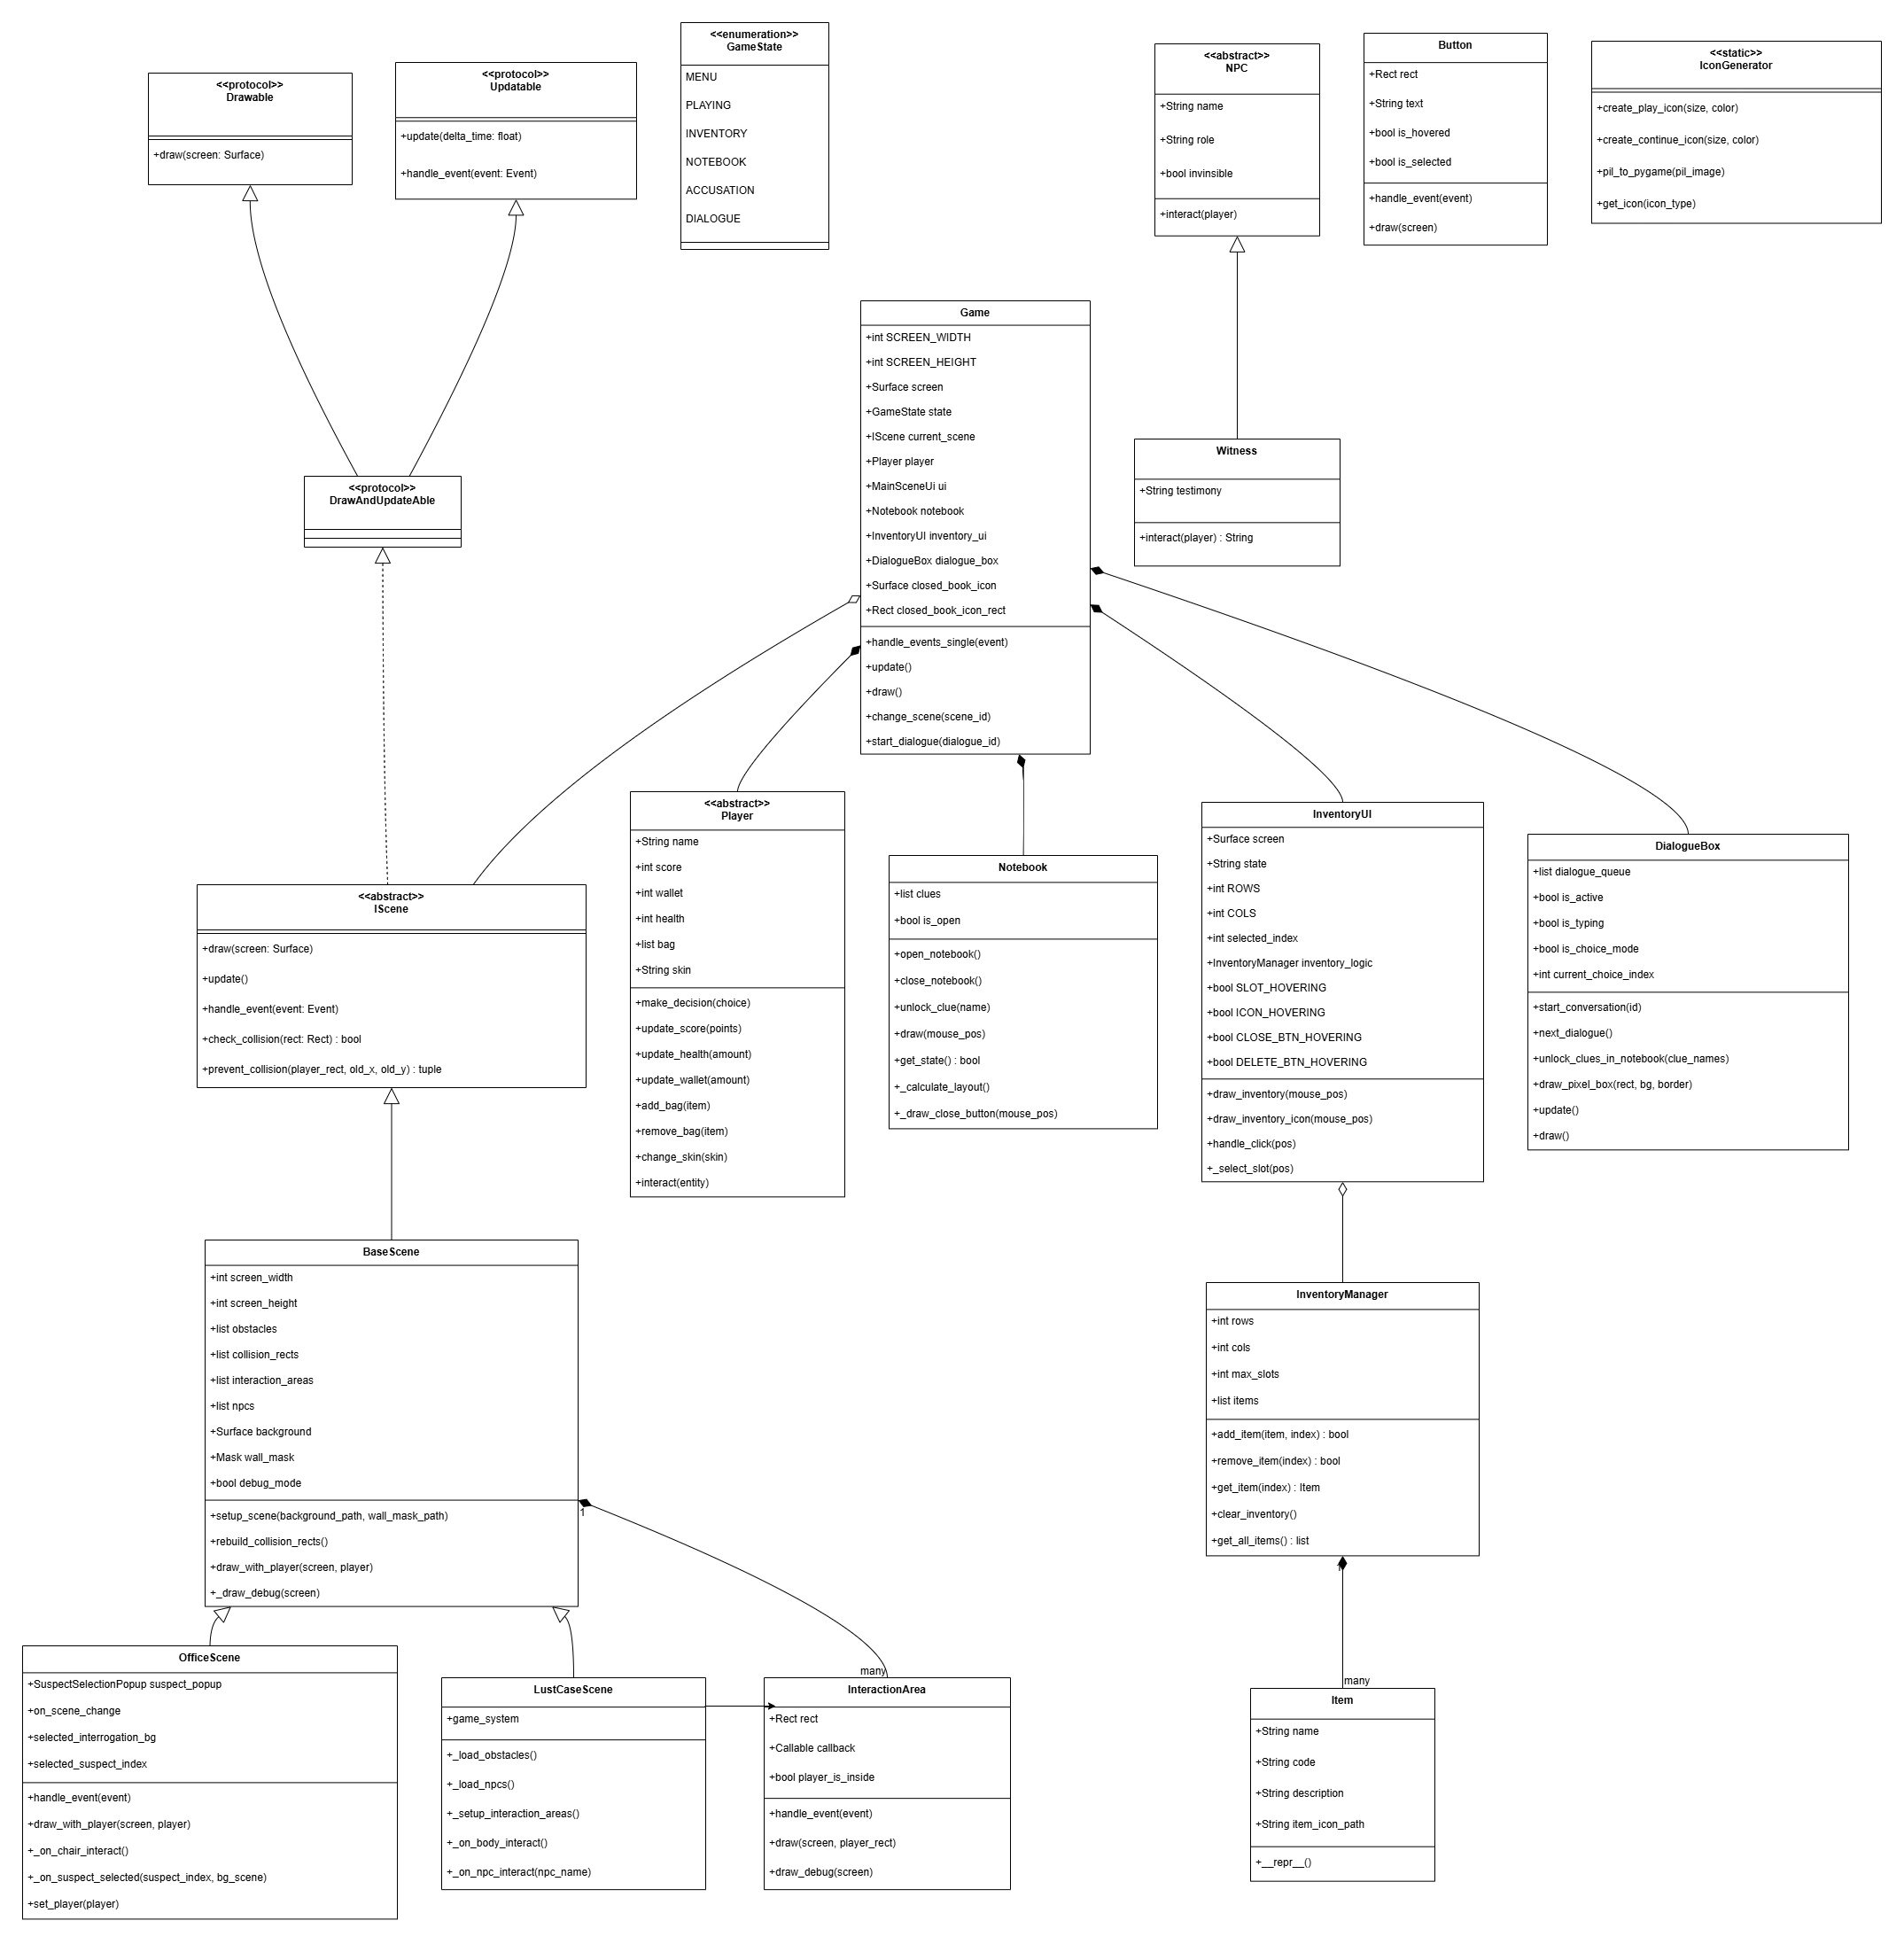
\includegraphics[width=\textwidth]{image/Diagram/Class.png} 
\end{figure}

\begin{description}

    \item[Lớp: Game] 
    Lớp trung tâm điều phối toàn bộ vòng lặp trò chơi (vẽ, cập nhật, xử lý sự kiện). Quản lý các thành phần chính như người chơi, cảnh hiện tại và chuyển đổi trạng thái giao diện.
    \begin{itemize}
        \item \textbf{handle\_events\_single(event) : void} \\
        Xử lý các sự kiện đầu vào (chuột, bàn phím) và phân luồng dựa trên trạng thái \texttt{GameState}.
        \item \textbf{change\_scene(scene\_id) : void} \\
        Thực hiện chuyển đổi giữa các màn chơi khác nhau và khởi tạo lại các tham chiếu cần thiết cho cảnh mới.
        \item \textbf{start\_dialogue(id) : void} \\
        Kích hoạt hệ thống hội thoại và nạp dữ liệu từ tệp cấu hình hội thoại.
    \end{itemize}

    \item[Lớp: BaseScene (Abstract)]
    Lớp trừu tượng cung cấp khung làm việc cơ bản cho mọi cảnh trong game, bao gồm quản lý hình ảnh nền và hệ thống va chạm.
    \begin{itemize}
        \item \textbf{setup\_scene(background, mask) : void} \\
        Tải tài nguyên hình ảnh nền và bản đồ va chạm (mask) để ngăn nhân vật đi xuyên tường.
        \item \textbf{draw\_with\_player(screen, player) : void} \\
        Vẽ cảnh và nhân vật theo thứ tự ưu tiên trục Y (Y-sorting) để tạo hiệu ứng chiều sâu 2D.
    \end{itemize}

    \item[Lớp: Notebook]
    Quản lý sổ tay ghi chép thám tử, lưu trữ và hiển thị các manh mối đã được người chơi thu thập.
    \begin{itemize}
        \item \textbf{unlock\_clue(name) : void} \\
        Tìm kiếm manh mối trong cơ sở dữ liệu và thay đổi trạng thái từ khóa sang hiển thị (\texttt{unlocked}).
        \item \textbf{\_calculate\_layout() : void} \\
        Tính toán vị trí các dòng chữ để nội dung luôn nằm khớp trên các đường kẻ của trang giấy trong sổ tay.
    \end{itemize}

    \item[Lớp: InventoryManager]
    Quản lý logic túi đồ, chịu trách nhiệm lưu trữ và thao tác trên mảng dữ liệu các vật phẩm.
    \begin{itemize}
        \item \textbf{add\_item(item, index) : bool} \\
        Thêm vật phẩm vào một ô cụ thể hoặc tìm ô trống đầu tiên. Trả về thành công hoặc thất bại.
        \item \textbf{remove\_item(index) : bool} \\
        Xóa dữ liệu vật phẩm tại vị trí được chỉ định để giải phóng ngăn chứa.
    \end{itemize}

    \item[Lớp: DialogueBox]
    Xử lý hiển thị hộp thoại, hiệu ứng chữ chạy và quản lý các lựa chọn của người chơi trong tương tác NPC.
    \begin{itemize}
        \item \textbf{next\_dialogue() : void} \\
        Chuyển sang đoạn thoại tiếp theo hoặc hiển thị danh sách lựa chọn nếu nhánh thoại kết thúc.
        \item \textbf{draw\_pixel\_box(rect, bg, border) : void} \\
        Vẽ hộp hội thoại theo phong cách Pixel Art với viền vàng và hiệu ứng đổ bóng đặc trưng.
    \end{itemize}

    \item[Lớp: InteractionArea]
    Định nghĩa một vùng không gian mà người chơi có thể tương tác khi đứng bên trong.
    \begin{itemize}
        \item \textbf{handle\_event(event) : void} \\
        Kiểm tra nếu người chơi nhấn phím \texttt{[F]} khi đang đứng trong vùng tương tác để kích hoạt hàm callback.
        \item \textbf{draw(screen, player\_rect) : void} \\
        Hiển thị chỉ dẫn tương tác lơ lửng phía trên đầu của nhân vật khi họ đi vào vùng này.
    \end{itemize}

\end{description}